\section{Zielsetzung}
Mit dem Franck-Hertz-Versuch soll die Quantennatur der Elektronenhülle,
wie sie durch das Bohrsche Atommodell, aber auch in der modernen Quantenmechanik,
postuliert wird, bestätigt werden. Dies soll dadurch gezeigt werden, dass Elektronen
in einem Gas beschleunigt werden. Wenn sich bei bestimmten Beschleunigungsspannungen die Zahl
ankommender Elektronen an der Anode abrupt deutlich reduziert, kann davon ausgegangen werden, dass das Gas erst bei einer diskreten 
Energie der Elektronen angeregt werden kann. Damit wäre gezeigt, dass Atome Energie nur 
quantisiert absorbieren können. Da ein angeregtes Atom nach einer kurzen Zeit in den Grundzustand
zurückfällt, emittiert das Quecksilber Photonen mit der gleichen Energiedifferenz, die es absorbiert hat.
Die entsprechende Wellenlänge soll in diesem Versuch ebenfalls ermittelt werden. Dafür muss zusätzlich das Kontaktpotential 
ermittelt werden und Frank-Hertz Kurven aufgenommen werden.
\section{Theorie}
\label{sec:Theorie}
Der Franck-Hertz-Versuch ist ein sogenanntes Elektronenstoßexperiment. Dabei werden Elektronen 
auf Atome geschossen, um anhand der Energiedifferenz vor und nach dem Stoß Informationen 
über die Elektronenhülle zu gewinnen. Für den Franck-Hertz-Versuch bedeutet das, dass 
möglichst monoenergetische Elektronen in einem abgeschlossenen Raum mit Quecksilber-Dampf wechselwirken.
Dabei treten bei niedrigen kinetischen Energien elastische Stöße auf. Dabei ändert sich auf Grund des großen Massenunterschieds 
kaum die kinetische Energie des Elektrons. Einzig die Bewegungsrichtung des Elektrons
ändert sich.\\
Beim unelastischen Stoß gibt das Elektron ein Teil seiner kinetischen Energie an das Quecksilber ab, 
um das Atom anzuregen, also ein Elektron in ein höheres Energieniveau zu heben.
Damit ergibt sich die Energiedifferenz der Elektronen nach dem Stoß zu
\begin{equation} 
    \frac{m\cdot v_\text{vor}^2}{2}-\frac{m\cdot v_\text{nach}^2}{2}=E_1-E_0.
    \label{eq:diff}
\end{equation}
Der generelle Aufbau des Franck-Hertz-Aufbau ist in Abbildung \ref{fig:FH} dargestellt.
Das Quecksilberdampf befindet sich in einem sonst evakuiertem Gefäß. Am Glühdraht ist eine Gleichspannung 
angeschlossen. Wenn der Glühdraht glüht, treten gemäß des glühelektrischen Effekts und dementsprechend
der Fermi-Dirac-Verteilung Elektronen aus. Diese haben im Allgemeinen alle unterschiedliche Energien.
In der Mitte der Apparatur ist eine netzförmige Anode. Zwischen Glühdraht und Anode wird 
eine Beschleunigungsspannung $U_\text{B}$ angeschlossen, die den Elektronen ihre ursprüngliche kinetische Energie geben.
Die Elektronen haben, solange sie nicht unelastisch gestoßen haben, die Energie
\begin{equation} 
    \frac{m\cdot v_\text{vor}^2}{2}=e_0U_\text{B}.
    \label{eq:ekin}
\end{equation}
Nun wird zwischen Anode und Auffangelektrode eine Gegenspannung $U_\text{A}$ angeschlossen. Mit dieser kann
die Energie der Elektronen die an der Anode ankommen bestimmt werden. Die Elektronen brauchen an der Anode noch die kinetische 
Energie, um das Gegenpotential zu überwinden. Es muss gelten 
\begin{equation}
    \label{eq:minE}
    \frac{m\cdot v_\text{z}^2}{2} \geq e_0U_\text{A},
\end{equation}
wobei $v_\text{z}$ die Geschwindigkeitskomponente in Feldrichtung beschreibt. Diese Bedingung
berücksichtigt keine elastischen Stöße zwischen Beschleunigungselektrode und Auffängerlektrode. Diese verfälschen 
das Ergebnis.\\
Jetzt gibt es verschiedene Bereiche zu diskutieren. Bei sehr geringen Beschleunigungsspannungen
ist die Ungleichung \eqref{eq:minE} nicht erfüllt und die Elektronen, die idealerweise monoenergetisch sind und beim Austritt aus der 
Elektrode keine kinetische Energie besitzen, können dann nicht das Gegenpotential überwinden.
Sobald die Ungleichung erfüllt ist, sollten die ersten Elektronen das Gegenpotential überwinden können und der 
Auffängerstrom sollte langsam anfangen zu steigen.
Wenn die Elektronen mehr kinetische Energie als die eines Schalenübergangs $E_1-E_0$ besitzen, stoßen 
die Elektronen unelastisch. Also sie geben den entsprechenden Energiebetrag gemäß 
Gleichung \eqref{eq:diff} an das Quecksilber ab. Dadurch reduziert sich die entsprechende kinetische Energie 
der Elektronen um die gleiche Energie. Diese Elektronen können das Gegenpotential zunächst wieder nicht 
überwinden. Erst bei noch größeren Beschleunigungsspannungen können die Elektronen das Gegenpotential wieder überwinden.
Dadurch ergibt sich idealisiert der Plot aus Abbildung \ref{fig:Diskret}. Es werden also periodische Zu- und Abnahmen 
des Auffängerstromes beobachtet. Der Abstand der Maxima muss dem zum Schalenübergang zugeordnetem
Potential
\begin{equation}
    U_1=\frac{E_1-E_0}{e_0}
    \label{eq:Anregungspotential}
\end{equation}
entsprechen, wobei das Quecksilberatom diese Energie in Form eine Photons mit der Energie $E_1-E_0$ abgibt.
Damit ergibt sich die Wellenlänge des Lichts in Abhängigkeit des Anregungspotentials aus Gleichung \eqref{eq:Anregungspotential} zu 
\begin{equation}
    \lambda =\frac{h\cdot c}{U_1\cdot e_0}.
    \label{eq:WellenL}
\end{equation}
\begin{figure}[H]
    \centering
    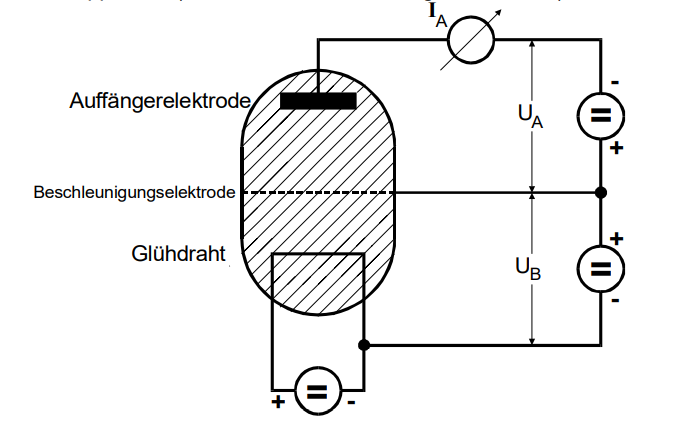
\includegraphics[scale=1]{content/PAufbau.png}
    \caption{Prinzipielle Aufbau des Frank-Hertz-Versuchs \cite{sample}.}
    \label{fig:FH}
\end{figure}

\begin{figure}[H]
    \centering
    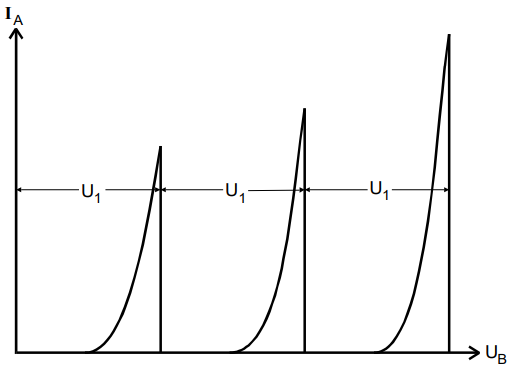
\includegraphics[scale=1]{content/Diskret.png}
    \caption{Idealisierter Zusammenhang zwischen Strom und Spannung \cite{sample}.}
    \label{fig:Diskret}
\end{figure}

\subsection{Einfluss des Kontaktpotentials}
Die angelegte Beschleunigungsspannung zwischen beiden Elektroden entspricht nicht direkt 
dem realen Beschleunigungspotential. Da der Glühdraht eine möglichst hohe Elektronenemissionsrate besitzen soll, ist 
ein Material gewählt worden mit einer deutlich geringeren Austrittsarbeit $\Phi_\text{G}$ als an der Beschleunigungselektrode $\Phi_\text{B}$.
Die entsprechenden Verhältnisse sind in Abbildung \ref{fig:KontaktU} abgebildet. Der entscheidende 
Einfluss auf die Messung besteht darin, dass das Beschleunigungspotential $U_\text{B}$ um
die Differenz der Austrittsarbeit, dem sogenannten Kontaktpotential, reduziert ist.
Das Kontaktpotential ergibt sich dann durch 
\begin{equation}
    K=\frac{\Phi_\text{B}-\Phi_\text{G}}{e_0}.
    \label{eq:Kontakt}
\end{equation}
Die effektiv wirkende Beschleunigungsspannung ist dann
\begin{equation}
    U_\text{B,eff}=U_\text{B}-K.
\end{equation}
\begin{figure}[H]
    \centering
    \includegraphics[scale=0.8]{content/Potentialverhältnisse.png}
    \caption{Potentialverhältnisse zwischen Glühkathode und Beschleunigungselektrode \cite{sample}.}
    \label{fig:KontaktU}
\end{figure}
\subsection{Einfluss des Energie-Spektrums der Elektronen}
Die ursprüngliche Annahme, dass alle Elektronen monoenergetisch sind, lässt sich in der 
Realität nicht halten. Die Elektronen besitzen bereits im Festkörper des Drahtes verschiedene Energien
gemäß der Fermi-Dirac-Verteilung. Dadurch haben die Elektronen bereits nach dem herauslösen 
aus dem Festkörper verschieden hohe kinetische Energien. Die langsamsten haben dabei nur die 
kinetische Energie des effektiven Beschleunigungspotential. Allerdings erstreckt sich die Energieverteilung mit abnehmender Häufigkeit 
auch über höhere Energien. Aus diesem Grund sind die Maxima nicht wie idealisiert angenommen 
scharf, sondern flach. Der Strom fängt schon vor der Spitze an weniger stark zuzunehmen und fällt auch nicht im Minimum auf 0 ab.
Ein weiterer Grund warum die Franck-Hertz-Kurve weniger scharf ausfällt, sind elastische Stöße im Zwischenbereich von 
Beschleunigungselektrode und Auffangelektrode. Die Stöße verändern zwar nicht die Energie, aber die Richtung und damit den relevanten Anteil 
der kinetischen Energie in Z-Richtung. Dadurch erreichen viele Elektronen, die es idealerweise bis zur Auffangelektrode geschafft hätten, diese 
nicht. Die Kurve flacht dadurch ab.
\subsection{Einfluss des Dampfdruckes}
Der Versuch basiert im Grunde auf der Wechselwirkung zwischen Elektronen und Atomen eines Gases durch Stöße.
Dabei sollte idealerweise jedes Elektron, wenn es die entsprechende kinetische Energie erreicht, mit 
einem Atom des Gases unelastisch stoßen. Andererseits sollen zu viele elastische Stöße, wie im vorherigen Abschnitt diskutiert, möglichst 
reduziert werden. Daher darf die freie Weglänge der Elektronen $\overline{w}$ wegen den gewünschten 
unelastischen Stößen nicht zu groß gewählt werden, aber auch nicht zu klein, da sonst zu viele ungewünschte elastische Stöße auftreten. Die freie Weglänge hängt 
gemäß der kinetischen Gastheorie vom Druck des Quecksilbers $p_\text{sät}$ durch 
\begin{equation}
    \overline{w}[\text{cm}]=\frac{0,0029}{p_\text{sät}}[\text{p in mbar}]
    \label{eq:freieW}
\end{equation}
ab. Das evakuierte Gefäß ist mit Tröpfchen von Quecksilber gefüllt. Ein Teil davon 
verdampft spontan bis sich ein Gleichgewicht gemäß der Dampfdruckkurve aus Abbildung 
\ref{fig:Dampf} einstellt. Dieser Sättigungsdampfdruck hängt dann nur von der Temperatur $T$ 
gemäß der Formel 
\begin{equation}
    p_\text{sät}=\qty{5.5e7}{\milli\bar}\cdot \text{e}^{-\qty{6876}{\kelvin}/T}
    \label{eq:Druck}
\end{equation}
ab. Optimalerweise wird die Temperatur der Franck-Hertz-Apparatur so eingestellt, dass die freie Weglänge etwa 
1000 bis 4000 mal kleiner ist als die Länge der Röhre. 
\begin{figure}[H]
    \centering
    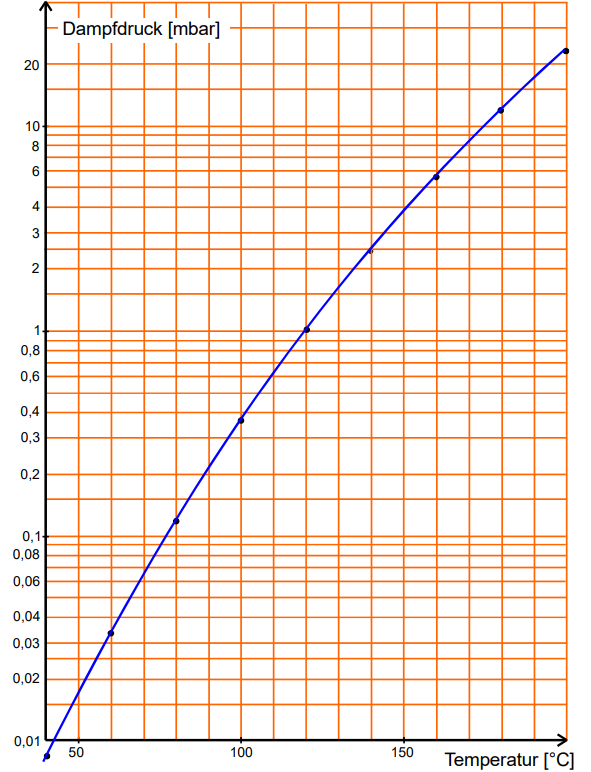
\includegraphics[scale=0.8]{content/Dampfdruckkurve.png}
    \caption{Dampfdruckkurve von Quecksilber \cite{sample}.}
    \label{fig:Dampf}
\end{figure}

\subsection{Aufbau der Hg-Elektronenhülle}
Von Spektroskopischer Bedeutung sind nur Elektronen in der äußersten Schale. Nur diese 
können überhaupt energetisch auf eine noch höhere nicht abgeschlossene Schale angehoben werden.
Im Falle von Quecksilber sind das 2 s-Elektronen mit Hauptquantenzahl $n=6$. Wegen des Pauli
Prinzips sind ihre Spins antiparallel. Der Grundzustand ist somit ein Singulett System ohne
Feinstruktur. Bei Anregung kann die S-Schale wie in Abbildung \ref{fig:Term} in 4 verschiedene Zustände
übergehen. Die potentielle Energie des Triplett Zustands ist auf Grund der 
parallelgestellten Elektronen geringer als bei Singulett Zustand. Bei einer normalen Anregung 
z.B. über ein einfallendes Photon müssten allerdings beide Spins parallel umklappen, was sehr unwahrscheinlich ist.
Beim Franck-Hertz-Versuch tritt das Problem nicht auf, da das Elektron das stößt durch das Elektron mit antiparallelem 
Spin austauschen kann. Da weniger potentielle Energie nötig ist um in diesen Zustand zu gelangen, ist dies der beobachtete Übergang.
\cite{sample}
\begin{figure}[H]
    \centering
    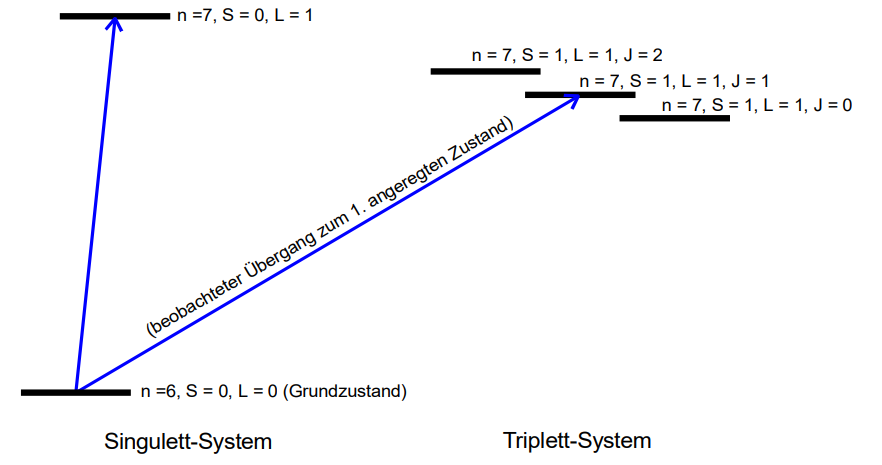
\includegraphics[scale=0.8]{content/Termschema.png}
    \caption{Termschema des Hg-Atoms \cite{sample}.}
    \label{fig:Term}
\end{figure}
